\documentclass[conference]{IEEEtran}

% Core
\usepackage{cite}
\usepackage{amsmath,amssymb,amsfonts}
\usepackage{graphicx}
\usepackage{booktabs}
\usepackage{makecell}
\renewcommand\theadfont{\normalsize\bfseries}
\usepackage{array}
\usepackage{multirow}
\usepackage{siunitx}
\usepackage{bm}
\usepackage{url}
\usepackage{hyperref}
\usepackage{xcolor}
\usepackage{algorithm}
\usepackage{algorithmic}

% Floats & subfigures
\usepackage{subcaption}
\usepackage{dblfloatfix}

\newcommand{\TODO}[1]{\textcolor{red}{\textbf{TODO:} #1}}

\title{Clearing Dense Log Piles with Imitation-Bootstrapped Reinforcement Learning}

\author{
Anonymous Authors
}
\begin{document}
\maketitle

\begin{abstract}
Clearing a dense pile of logs by sequential grasping is a contact-rich manipulation problem. The scene contains hundreds of rigid bodies in frictional contact, each grasp reshapes the pile, and effective strategies span long horizons.
We study this problem in simulation for a forestry log loader that must clear piles of 200 logs using only depth-derived point clouds requiring no semantic segmentation.
From-scratch reinforcement learning (RL) fails to discover effective clearing strategies regardless of observation type.
Our framework first trains a PointNet-based policy via behavior cloning (BC) on demonstrations from a privileged-state heuristic, then fine-tunes with RL using an asymmetric actor-critic.
BC provides the full-trajectory exploration curriculum that RL alone cannot discover, while RL optimizes per-grasp quality beyond what the demonstrator achieves.
The resulting policy maintains expert-level clearing ($98.2$\%) while improving grasp stability by $15$\% over the BC initialization, using only depth-derived point clouds.
\end{abstract}

\begin{IEEEkeywords}
robot learning, multi-object grasping from dense clutter, behavior cloning, reinforcement learning fine-tuning, contact-rich simulation
\end{IEEEkeywords}

\section{Introduction}
Forestry operations increasingly seek autonomy for heavy machinery to improve safety and productivity~\cite{lindroos2015forestry}.
A key subtask is log-pile clearing: repeatedly grasping multiple logs from a rack or pile and removing them.
This setting is challenging because (i) the scene is densely cluttered with hundreds of rigid-body logs in frictional contact, (ii) each grasp disturbs the pile through contact cascades, continuously reshaping the configuration for subsequent attempts, and (iii) no two pile configurations are alike, so a targeting strategy must be robust to diverse arrangements.

We address the grasp target selection problem: given a raw point cloud derived from a stereo depth camera, where should the crane place and orient the grapple to clear the pile efficiently?
We deliberately separate this high-level targeting decision from low-level motion execution.
Concretely, we implement a grasp-and-remove simulator in Isaac Lab~\cite{mittal2023orbit} where each environment step is one complete pick attempt: a policy selects where to grasp, a fixed FSM handles execution, and grasped logs are removed rather than deposited, allowing us to measure clearing progress without modeling placement dynamics.

Existing work on autonomous log grasping addresses small-scale settings: single-log pick-and-place, small groupings of 2--7 logs, or grasp prediction without sequential clearing.
We scale to full pile-level clearing with dense frictional contact dynamics among hundreds of logs.
To our knowledge, this is the first study of learned sequential grasp targeting at this pile scale.

Dense log-pile clearing poses a difficult exploration problem for reinforcement learning: reward signal is sparse across long episodes of sequential grasps, and the high-dimensional point-cloud observation space compounds the challenge.
We find that from-scratch RL stalls at roughly 53\% pile clearing, a failure that persists across all observation types tested.
Our approach is to first train a policy via behavior cloning (BC) on demonstrations from a privileged-state heuristic, then fine-tune with RL.
The demonstration data spans the complete clearing trajectory, giving the RL agent the distributional coverage it cannot acquire through its own exploration.

Our main contributions are:
\begin{itemize}
    \item A BC$\to$RL fine-tuning pipeline in which a PointNet encoder, pretrained via BC on heuristic demonstrations from raw point clouds, is frozen during RL while only the policy head is updated with an asymmetric actor-critic~\cite{pinto2018asymmetric} that pairs the vision-based actor with a privileged-state critic. This prevents catastrophic forgetting of the learned visual features while letting RL optimize per-grasp execution. The resulting policy surpasses the privileged-state expert in grasp stability using depth alone.
    \item A grasp-and-remove crane environment in Isaac Lab for dense pile clearing at scale (200 logs), with a fixed FSM that isolates targeting from execution and supports GPU-parallelized training.
    \item A four-method comparison showing: (a) from-scratch RL fails regardless of observation type, (b) BC achieves near-expert clearing from raw point clouds, and (c) BC+RL improves grasp stability by 15\% while maintaining clearing performance.
\end{itemize}

\section{Related Work}

\subsection{Grasping in Clutter}
Learning-based grasp detection has progressed from single isolated objects to cluttered, multi-object scenes, with applications spanning industrial bin picking of manufactured parts~\cite{mahler2017dexnet}, warehouse depalletizing~\cite{zeng2018learning}, and natural-resource handling such as forestry log loading~\cite{wallin2024multilog}.
Deep grasp prediction networks~\cite{morrison2018closing, kumra2017robotic} predict grasp pose directly from visual input.
Sequential decluttering has been studied in bin picking~\cite{mahler2017dexnet, zeng2018learning}, including learning grasp sequences that account for how each pick changes the scene~\cite{mahler2017sequential}.
However, these works typically involve heterogeneous objects of varied shape and size in loose arrangements, where clutter arises from random placement rather than dense packing.
The grasping primitive is almost always a precision or pinch grasp that isolates a single target object.
Our setting differs in important ways: we perform power grasps from dense piles of cylindrical logs of uniform geometry that are initially stacked in ordered layers.
The homogeneity and tight packing mean that logs are in extensive frictional contact with their neighbors, and each grasp attempt (which captures multiple logs simultaneously) disturbs the pile, causing settling, rolling, and potential knock-offs that reshape the configuration for all subsequent attempts.
For 3D perception of unordered point sets, PointNet~\cite{qi2017pointnet} and its variants provide a natural encoder architecture.

\subsection{Learning for Log Grasping and Forestry Crane Control}
A growing body of work applies learning methods to log grasping and forestry crane automation, though existing approaches address smaller-scale settings than the one considered here.

For grasp prediction, Wallin et~al.~\cite{wallin2024multilog} use RL with virtual visual servoing for multi-log grasping from small groupings of 2--5 logs in simulation, separating image segmentation from Cartesian crane control; their agent achieves 95\% success but the pile dynamics are limited to a handful of objects.
F{\"a}lldin et~al.~\cite{falldin2025synthesizing} train a U-Net CNN on synthetic RGB-D images to predict grasp poses for small clusters of up to 7 logs, with an open-loop kinematic controller; their work focuses on grasp prediction from synthetic data and does not address sequential clearing or pile-scale dynamics.
Ayoub et~al.~\cite{ayoub2023grasp} propose a CNN-based grasp planner for a log-loading forestry machine that predicts a grasp configuration from a depth image for small piles, validated both in simulation and on a commercial log loader retrofitted for autonomy.

For crane control, Vu et~al.~\cite{vu2025autonomous} present a MuJoCo-based forestry crane simulator and benchmark RL velocity controllers for grasping single logs of varying diameter (simulation only).
Kurinov et~al.~\cite{kurinov2025reinforcement} train an RL agent for the full single-log pick-and-place pipeline (locate, grasp, transport, load) in Isaac Gym simulation, achieving 94\% success across parallel environments but with one log at a time.
Jebellat et~al.~\cite{jebellat2025designing} use dynamic programming to design anti-sway trajectories for a log loader end effector, addressing the pendulum dynamics that also arise in our passive grapple chain.
These works address individual subtasks but none tackle sequential clearing of a dense pile at the scale considered here.

More broadly, using demonstrations to initialize RL policies has been shown to overcome exploration challenges in contact-rich manipulation~\cite{rajeswaran2018learning, nair2018overcoming}, and asymmetric actor-critic architectures (where the critic receives privileged state information unavailable to the actor) have proven effective for learning from high-dimensional visual observations~\cite{pinto2018asymmetric}.
To our knowledge, no prior work combines these ideas for sequential pile clearing from point clouds.

\section{Task Formulation}
\subsection{Grasp-and-Remove Formulation}
\label{sec:formulation}
Each environment step corresponds to a complete grasp attempt: a policy selects a grasp target, the FSM executes the approach, close, and lift, and grasped logs are removed from the scene.
This formulation is shared by all methods (heuristic, BC, RL, and BC+RL).
The state $s_t \in \mathcal{S}$ is the current pile configuration (observed via point cloud or privileged poses; Section~\ref{sec:obs}).
A grasp target is defined by the tuple
\begin{equation}
    \mathbf{g} = (x,\, y,\, z,\, \psi),
\end{equation}
where $(x, y, z)$ is the grapple position in the crane base frame and $\psi$ is the grapple yaw angle about the vertical axis.
Because a cylindrical log at yaw $\psi$ is identical to the same log at $\psi + \pi$, the policy represents $\psi$ via the $\pi$-periodic encoding $(\cos 2\psi, \sin 2\psi)$~\cite{morrison2018closing}, giving a 5D action $a_t \in \mathcal{A} \subset \mathbb{R}^5$ (Section~\ref{sec:actions}).
The transition $T(s_{t+1}|s_t, a_t)$ is determined by the physics simulation and FSM execution.
After each grasp attempt, an outcome evaluation measures the number of logs grasped, grapple--log alignment, and grapple stability (Section~\ref{sec:outcome}).
For RL training, this outcome is used as a scalar reward $r_t = R(s_t, a_t)$, and the full structure is treated as an episodic Markov decision process $(\mathcal{S}, \mathcal{A}, T, R, \gamma)$ with discount factor $\gamma$, where a policy $\pi$ maximizes the expected discounted return over a horizon of $H$ grasp attempts:
\begin{equation}
    \max_\pi \; \mathbb{E}_\pi \!\left[\sum_{t=0}^{H-1} \gamma^t \, r_t \right].
\end{equation}
An episode terminates when no logs remain on the rack or after a fixed horizon of $H=30$ grasp attempts.
A log leaves the rack either by being grasped and removed or by being knocked outside the workspace bounds (Section~\ref{sec:outcome}); both reduce the remaining count for termination purposes, but only intentionally grasped logs are credited toward the clearing rate metric (Section~\ref{sec:metrics}).
The horizon is chosen to exceed the minimum needed: the grapple can hold up to 20 logs per grasp, and the heuristic baseline clears 200-log piles in approximately 20 attempts, so $H=30$ provides a 50\% margin while keeping episodes tractable.


\subsection{Observations}
\label{sec:obs}
The policy observes a raw point cloud of the scene.
A depth camera mounted on the crane renders the scene from above the rack, producing a depth image $D_t$.
The simulated camera uses a pinhole model with parameters matching the Stereolabs ZED~X in wide-angle configuration\footnote{\url{https://www.stereolabs.com/products/zed-x}}.

The observation is constructed in three steps (Fig.~\ref{fig:pcd_pipeline}).
First, each pixel $(u,v)$ with a valid depth reading within the sensor range is back-projected to a 3D point using the camera intrinsic matrix $\mathbf{K} \in \mathbb{R}^{3 \times 3}$:
\begin{equation}
    \mathcal{P}_w = \big\{\, \mathbf{K}^{-1}(u,v,1)^\top \!\cdot D_t(u,v) \;\big|\; d_{\min} \le D_t(u,v) \le d_{\max} \big\},
\end{equation}
where the camera-frame points are transformed to the world frame using the known camera extrinsics.
Second, each point $\mathbf{p} \in \mathcal{P}_w$ is transformed into the crane base frame using the base-frame rotation $\mathbf{R}_b$ and translation $\mathbf{t}_b$:
\begin{equation}
    \mathcal{P}_b = \big\{\, \mathbf{R}_b^\top(\mathbf{p} - \mathbf{t}_b) \;\big|\; \mathbf{p} \in \mathcal{P}_w \big\}.
\end{equation}
Third, Farthest Point Sampling (FPS) downsamples $\mathcal{P}_b$ to a fixed-size set of $N_p = 1024$ points, yielding the observation:
\begin{equation}
    o_t = \mathrm{FPS}(\mathcal{P}_b,\; N_p) \;\in \mathbb{R}^{N_p \times 3}.
\end{equation}
If the cloud contains fewer than $N_p$ points (e.g., near the end of an episode), the remaining rows are zero-padded.
Crucially, no semantic segmentation is applied: the raw point cloud includes all surfaces visible to the depth camera (logs, rack, ground).
The PointNet encoder must implicitly learn to attend to task-relevant geometry.
We compare raw and segmented point clouds in Section~\ref{sec:results}.

As an ablation, we also evaluate policies that observe privileged per-object state: the top-$K$ log poses sorted by height (highest first), each represented as $(x,y,z,\psi)$ in the crane base frame.
Removed logs are excluded and remaining slots are padded with $-1$.
With $K\!=\!32$ this yields a compact $4K = 128$ dimensional vector.
This baseline isolates the effect of the perception gap: any performance difference between pose and point cloud policies is attributable to the observation representation rather than the learning algorithm.

\subsection{Actions and Workspace Scaling}
\label{sec:actions}
The policy outputs a 5D vector $\tilde{a}_t \in \mathbb{R}^5$ (before squashing).
The first three components encode position and the remaining two encode grapple yaw via a cosine--sine pair.

Each position component is squashed via the hyperbolic tangent $\tanh$ and then linearly mapped to the per-environment workspace bounds to produce the target coordinate $p_i$:
\begin{equation}
    p_i = \frac{(\tanh \tilde{a}_i + 1)}{2}(b_i^{\max} - b_i^{\min}) + b_i^{\min}, \quad i \in \{x,y,z\},
\end{equation}
where $b_i^{\min}, b_i^{\max}$ are the rack-aligned workspace limits for each axis.
These bounds are derived from the rack geometry with margins along each axis.
The resulting workspace is approximately $2.0 \times 5.2 \times 1.0$\,m in the crane base frame.
The bounds serve a dual purpose.
First, they define the policy's reachable target space, ensuring that all output actions map to physically executable grasp poses.
Second, logs that drift outside these bounds during a grasp attempt (e.g., knocked off the rack by grapple contact) are automatically removed before the next targeting decision and counted separately (see Section~\ref{sec:outcome}), preventing unreachable logs from accumulating.
The heuristic expert (Section~\ref{sec:expert}), which bypasses the policy's action scaling and targets log poses directly, operates within the same spatial bounds.

The remaining two components encode the grapple yaw angle $\psi$ about the vertical axis.
A cylindrical log at yaw $\psi$ is physically identical to the same log at $\psi + \pi$.
A scalar representation forces the network to learn this symmetry from data; instead, following the grasp-angle encoding of Morrison et~al.~\cite{morrison2018closing}, we encode $\psi$ as the pair $(\cos 2\psi,\;\sin 2\psi)$, which has period $\pi$ and thus maps symmetric orientations to the same point.
The policy outputs two scalars $(\tilde{a}_4, \tilde{a}_5)$; after squashing, the yaw is recovered as
\begin{equation}
    \psi = \tfrac{1}{2}\,\mathrm{atan2}\!\big(\tanh \tilde{a}_5,\;\tanh \tilde{a}_4\big) \;\in \big[-\tfrac{\pi}{2},\;\tfrac{\pi}{2}\big].
\end{equation}

For BC training, expert targets are encoded in the same space: positions are normalized and passed through $\mathrm{arctanh}$, and yaw is stored directly as $(\cos 2\psi, \sin 2\psi)$.
This ensures BC and RL policies operate in an identical action space.

\section{Environment and Controller}
\subsection{Low-level Execution FSM}
All methods share the same fixed FSM controller, which runs at the control rate (60\,Hz, i.e., 120\,Hz physics with $2\times$ decimation) inside each environment step.
Given a grasp target $(x,y,z,\psi)$, produced by the heuristic (Section~\ref{sec:expert}) or a learned policy (BC or RL), the FSM executes a complete grasp cycle.

The crane arm has four actuated joints (basemast, boom, stick, and telescope) followed by a two-link passive chain that suspends the grapple from the telescope tip.
The two passive joints are unactuated revolute joints with low stiffness and damping, modeling the gravity-driven hanging behavior of a real forestry crane's grapple attachment.
Below the passive chain, a yaw joint actively rotates the grapple about the vertical axis, and two gripper joints control the jaw opening.

In this kinematic structure, the IK controller commands the top of the passive chain, but the grapple body hangs $\sim$0.4\,m below it and swings like a pendulum during arm movements.
Consequently, all grasp targets are specified for the grapple body and then offset vertically to the IK target link.
The FSM uses a two-stage convergence check at each phase: it first waits for the IK target link to reach its target within $\epsilon_{\text{up}} = 0.10$\,m, then waits for the grapple body to settle within $\epsilon_{\text{bg}} = 0.25$\,m.
Both must hold for $N_{\text{dwell}} = 30$ consecutive timesteps before the phase advances, ensuring that pendulum oscillations have damped before proceeding.

The FSM implements a five-phase grasp cycle:
\begin{enumerate}
    \item \texttt{HOVER}: Move grapple to hover position above the target $(x, y, z + z_{\text{clear}})$, with $z_{\text{clear}} = 2.5$\,m clearance above the target log.
    \item \texttt{ALIGN}: Hold position and rotate grapple to the target yaw $\psi$.
    \item \texttt{DESCEND}: Lower grapple to approach height at reduced speed (30\% step scaling) to minimize pile disturbance.
    \item \texttt{CLOSE}: Close the grapple jaws incrementally via discrete stepping.
    \item \texttt{LIFT}: Lift back to hover height at moderate speed (50\% step scaling), then hold for $\sim$1\,s while grasp outcome is evaluated (Section~\ref{sec:outcome}). Grasped logs are removed, the jaws open, and the cycle repeats from \texttt{HOVER} with the next target.
\end{enumerate}
A per-phase timeout (100 timesteps, $\sim$2\,s) forces advancement if the two-stage convergence is not reached, preventing the FSM from stalling on difficult configurations.

The arm is controlled using Isaac Lab's task-space Differential IK controller~\cite{mittal2023orbit} (damped least-squares, position command type), which computes joint position targets from the current end-effector pose and Jacobian.
The grapple yaw joint is controlled independently via a PD position controller.
The grapple jaws are controlled using a PD velocity law with saturation and discrete stepping to avoid abrupt contact forces.

\subsection{Outcome Evaluation}
\label{sec:outcome}
After lifting (\texttt{LIFT}), the FSM holds the grapple at hover height and evaluates grasp outcome by measuring proximity and orientation of logs relative to the \texttt{basegrapple} body:
\textbf{Logs grasped} ($g$): the number of active logs (i.e., logs not yet removed from the scene) whose centers lie within a proximity radius of the grapple (default 1.5\,m).

\textbf{Alignment} ($\alpha$): for each grasped log $i$, we measure the angle between the grapple's jaw axis $\hat{y}_g$ and the log's length axis $\hat{y}_{\ell_i}$ via their dot product ($\hat{y}_g^\top \hat{y}_{\ell_i} = \cos\theta_a$, where $\theta_a$ is the misalignment angle).
Because a cylindrical log has no preferred length direction, the even exponent absorbs the sign; raising to the 8th power creates a sharp dropoff that penalizes moderate misalignment:
\begin{equation}
    \alpha_i = \big(\hat{y}_g^\top \hat{y}_{\ell_i}\big)^{8}, \qquad \alpha = \frac{1}{g}\sum_{i=1}^{g} \alpha_i \;\in [0,1].
\end{equation}

\textbf{Stability} ($\varsigma$): the grapple's levelness after lifting, measured as $\hat{z}_g^\top \hat{z}_w = \cos\theta_s$, where $\theta_s$ is the tilt angle between the grapple's up vector and the world vertical.
Clamping to zero excludes the degenerate case of an inverted grapple; raising to the 4th power ensures high scores only when the grapple is nearly level:
\begin{equation}
    \varsigma = \big(\max(0,\;\hat{z}_g^\top \hat{z}_w)\big)^{4} \;\in [0,1].
\end{equation}
We define \textbf{grasp quality} as the product $q = \alpha \cdot \varsigma \in [0,1]$, capturing how well-aligned and stable a grasp is independently of how many logs were captured.

Logs identified as grasped are marked inactive and teleported out of the scene.
Logs that leave the workspace bounds during a grasp are removed and excluded from the grasp count $g$.
Figure~\ref{fig:grasp_geometry} visualizes the shaped score curves for alignment and stability.

\begin{figure}[t]
\centering
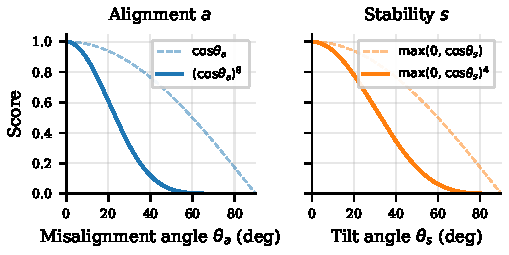
\includegraphics[width=\columnwidth]{outcome_scores.pdf}
% TODO: Add geometric diagram panel (crane/grapple with coordinate frames, action space bounding box) alongside the score curves.
\caption{Grasp geometry and action space. Left: coordinate frames used to compute alignment ($\alpha$) and stability ($\varsigma$). The alignment score measures parallelism between the grapple jaw axis $\hat{y}_g$ and the log length axis $\hat{y}_\ell$; stability measures the grapple's levelness via $\hat{z}_g^\top \hat{z}_w$. Right: the 3D workspace bounds define the policy's action space over the rack.}
\label{fig:grasp_geometry}
\end{figure}

We implement the environment in Isaac Lab and run PhysX GPU dynamics for scalable data collection.
Log and contact parameters (Table~\ref{tab:sim_params}) are based on measurements of representative forestry logs and published friction coefficients for oak on oak~\cite{avallone2006marks}.
We use conservative contact modeling (simplified collision geometry on the grapple, tuned contact and rest offsets, and damping limits for logs) to reduce interpenetration and numerical jitter while maintaining high throughput.


\begin{table}[t]
\centering
\caption{Simulation and controller parameters. Actuator gains are implicit PhysX joint-drive values; IK gains are the PD velocity controller used by the FSM.}
\label{tab:sim_params}
\setlength{\tabcolsep}{3pt}
\small
\begin{tabular}{@{}lr@{}}
\toprule
\multicolumn{2}{l}{\textit{Simulation}} \\[2pt]
Physics timestep ($\Delta t$) & $1/120$ s \\
Control decimation & $2\times$ (60 Hz) \\
\addlinespace[4pt]
\multicolumn{2}{l}{\textit{Crane link masses}} \\[2pt]
Mast / Main boom / Stick & 290 / 172 / 70 kg \\
Telescope / Upperpassive & 25 / 9 kg \\
\addlinespace[4pt]
\multicolumn{2}{l}{\textit{Joint limits}} \\[2pt]
Basemast (revolute) & $\pm100^{\circ}$ \\
Boom (revolute) & $-22^{\circ}$ to $+75^{\circ}$ \\
Stick (revolute) & $-177^{\circ}$ to $+2^{\circ}$ \\
Telescope (prismatic) & 0.13--1.80 m \\
Grapple (revolute) & $\pm180^{\circ}$ \\
\addlinespace[4pt]
\multicolumn{2}{l}{\textit{Actuator gains} ($k_p$ / $k_d$)} \\[2pt]
Main arm joints & $10^{6}$ / $10^{5}$ \\
Passive chain & 300 / 500 \\
Grapple yaw & $5\!\times\!10^{4}$ / $2\!\times\!10^{4}$ \\
Grapple tongs & 0 / 500 \\
\addlinespace[4pt]
\multicolumn{2}{l}{\textit{IK controller PD gains} ($k_p$ / $k_d$)} \\[2pt]
Arm joints & 4.0 / 1.2 \\
Grapple tongs & 12.0 / 1.0 \\
\addlinespace[4pt]
\multicolumn{2}{l}{\textit{FSM parameters}} \\[2pt]
Hover clearance & 2.5 m \\
Position tol.\ (upperpassive / basegrapple) & 0.10 / 0.25 m \\
Dwell count & 30 steps \\
Phase timeout & 100 steps \\
\addlinespace[4pt]
\multicolumn{2}{l}{\textit{Log properties}} \\[2pt]
Diameter / length & $\sim$0.3 / $\sim$3.0 m \\
Mass & 15 kg \\
Static / kinetic friction ($\mu_s$ / $\mu_k$) & 0.62 / 0.48 \\
Angular damping & 0.05 \\
Contact / rest offset & 0.02 / 0.0 m \\
Max depenetration velocity & 3.0 m/s \\
\bottomrule
\end{tabular}
\end{table}

\section{Baseline and Learned Policies}

\subsection{Heuristic Expert}
\label{sec:expert}
We implement a hand-tuned heuristic expert that serves both as a competitive baseline and as the demonstration source for BC.
The heuristic has access to privileged information (the position and orientation of every active log from the physics engine) and uses a deterministic top-of-pile targeting strategy:

At the start of each pick cycle (\texttt{HOVER} phase), the expert queries the simulator for the world-frame poses of all active logs in the environment.
It selects the log with the highest $z$-coordinate (i.e., the topmost log in the pile), transforms its center position into the crane base frame, and sets this as the $(x,y,z)$ grasp target.
This greedy rule is effective because the highest log is typically the most accessible; it has the fewest obstructing neighbors and the grapple can reach it with minimal contact disturbance to the surrounding pile.

After positioning the grapple above the target, the expert computes an optimal yaw $\psi$ that aligns the grapple's jaw axis with the target log's principal (length) axis.
The target log's yaw is extracted from its world-frame quaternion and transformed into the crane base frame.
Because a cylindrical log at yaw $\psi$ is symmetric with the same log at $\psi + \pi$, the expert evaluates both orientations and selects the one requiring minimal joint rotation from the current configuration.
This alignment is recomputed in the \texttt{ALIGN} phase using the grapple's live orientation, providing closed-loop yaw tracking rather than open-loop targeting.

The expert's greedy strategy is effective for dense piles: when many logs are stacked, the highest log is reliably graspable, and good alignment ensures that the grapple captures neighboring logs along the same layer.
However, the heuristic makes no multi-step plan.
In the endgame, when only a few scattered logs remain, targeting the highest log is no longer clearly optimal; logs may be isolated, partially wedged, or positioned where the grapple geometry makes alignment difficult.
Despite this, the expert achieves strong performance across all metrics (Table~\ref{tab:results}).

\subsection{Behavior Cloning}
\label{sec:bc}
We use BC~\cite{pomerleau1988alvinn} to train a policy from expert demonstrations.
We collect demonstration pairs $(o_t, a_t)$ from successful expert grasps only (failed grasps are discarded), where $o_t$ is the point cloud observation and $a_t$ is the expert action in the pre-squashing space (positions via $\mathrm{arctanh}$, yaw via $\cos 2\psi, \sin 2\psi$ as described in Section~\ref{sec:actions}).

The policy uses a PointNet encoder~\cite{qi2017pointnet}.
A shared per-point MLP $h: \mathbb{R}^3 \to \mathbb{R}^{256}$ (layers $3 \!\to\! 64 \!\to\! 128 \!\to\! 256$ with batch normalization and ELU activations) maps each point independently; a symmetric max-pool aggregates the per-point features into a global latent vector:
\begin{equation}
    \mathbf{z} = \max_{i=1,\ldots,N_p} h\!\big(o_t^{(i)}\big) \;\in \mathbb{R}^{256},
\end{equation}
where $o_t^{(i)} \in \mathbb{R}^3$ is the $i$-th point in the observation.
An actor MLP $\mu_\theta: \mathbb{R}^{256} \to \mathbb{R}^{5}$ (layers $256 \!\to\! 128 \!\to\! 64 \!\to\! 5$) maps the latent to the action $\tilde{a}_t = \mu_\theta(\mathbf{z})$.
For the privileged-pose ablation, we replace the PointNet encoder with a three-layer MLP ($128 \!\to\! 256 \!\to\! 128 \!\to\! 64$) with ELU activations.

Table~\ref{tab:architecture} summarizes the network architecture for both observation types.

\begin{table}[t]
\centering
\caption{Network architectures. All hidden layers use ELU activations. The PointNet encoder applies batch normalization. All policies output 5D actions: $(x,y,z,\cos 2\psi,\sin 2\psi)$.}
\label{tab:architecture}
\setlength{\tabcolsep}{3pt}
\begin{tabular}{@{}lp{2.4cm}p{2.4cm}p{2.0cm}@{}}
\toprule
& \textbf{BC / RL (PCD)} & \textbf{BC+RL (PCD)} & \textbf{RL (Pose)} \\
\midrule
Encoder
  & PointNet: $3\!\to\!64\!\to\!128\!\to\!256$, BN, max-pool
  & Same (frozen, init from BC)
  & MLP: $128\!\to\!256\!\to\!128\!\to\!64$ \\[3pt]
Actor
  & $256\!\to\!128\!\to\!64\!\to\!5$
  & Same (init from BC)
  & Shared enc $\to$ $64\!\to\!5$ \\[3pt]
Critic
  & PointNet + MLP head
  & MLP: $128\!\to\!256\!\to\!128\!\to\!1$ (state)
  & MLP: $256\!\to\!128\!\to\!64\!\to\!1$ \\
\bottomrule
\end{tabular}
\end{table}

We apply dropout (rate 0.2) after the encoder.
The BC objective minimizes the mean-squared error between the predicted and expert actions over a dataset $\mathcal{D}$ of successful grasps:
\begin{equation}
    \mathcal{L}_{\text{BC}} = \frac{1}{|\mathcal{D}|}\sum_{(o,a^*)\in\mathcal{D}} \left\| \mu_\theta(\mathbf{z}) - a^* \right\|^2,
\end{equation}
where $\mathbf{z}$ is the encoder output for observation $o$.
We optimize with AdamW~\cite{loshchilov2019adamw} (learning rate $10^{-4}$, weight decay $10^{-4}$) and ReduceLROnPlateau scheduling (factor 0.5, patience 10 epochs).
The training dataset contains $\sim$20{,}700 successful-grasp samples ($\sim$85/15 train/validation split). The raw PCD model is selected by minimum validation loss (0.101 MSE, epoch 190) with early stopping (patience 30 epochs).

\subsection{Reinforcement Learning}
\label{sec:rl}
We train policies with PPO~\cite{schulman2017ppo} using the RSL-RL library~\cite{rudin2022learning}.
PPO optimizes a stochastic Gaussian policy with parameters $\theta$:
\begin{equation}
    \pi_\theta(a \mid s) = \mathcal{N}\!\big(\mu_\theta(s),\;\mathrm{diag}(\bm{\sigma}^2)\big),
\end{equation}
where $\mu_\theta$ outputs the mean action and $\bm{\sigma} \in \mathbb{R}^{|\mathcal{A}|}$ is a learnable standard deviation vector controlling exploration noise, initialized to $\sigma_0$ and updated by gradient descent alongside the actor weights.
A separate critic network estimates the state-value function:
\begin{equation}
    V_\phi(s) \approx \mathbb{E}_\pi\!\left[\sum_{t'=t}^{H-1} \gamma^{t'-t}\, r_{t'} \;\Big|\; s_t = s\right],
\end{equation}
with parameters $\phi$ trained to minimize the prediction error against observed returns.
Advantages are computed via Generalized Advantage Estimation (GAE)~\cite{schulman2017ppo}.

The actor uses the same PointNet encoder and actor MLP as the BC policy; the critic uses an independent PointNet encoder with its own MLP head.
For the privileged-pose ablation, both actor and critic are separate MLPs with hidden dimensions $[256, 128, 64]$ and ELU activations.
Key hyperparameters: $\sigma_0 = 1.0$, clipping ratio $\epsilon=0.2$, entropy coefficient $0.01$, learning rate $3\times10^{-4}$ with adaptive KL-based scheduling (target KL $0.01$), GAE with $\lambda=0.95$, discount factor $\gamma = 0.99$, 4 steps per environment per iteration, 5 learning epochs with 4 mini-batches per epoch, and gradient clipping at norm $1.0$.
Each iteration collects $N_{\text{env}} \times 4$ grasp cycles (one step per cycle) across all parallel environments and performs one PPO update; total grasp experience after $k$ iterations is therefore $4 k N_{\text{env}}$.
The outcome components $(g,\alpha,\varsigma)$ from Section~\ref{sec:outcome} define the scalar reward:
\label{eq:reward}
\begin{equation}
r = g \cdot \alpha \cdot \varsigma = g \cdot q,
\end{equation}
for successful grasps ($g > 0$), and $r = \rho_{\text{fail}} = -1$ for failed grasps.
The reward is thus the product of throughput and grasp quality; a high reward requires many logs grasped with good alignment and a level grapple.
The reward is entirely per-grasp.
Global pile-clearing ability must emerge from the policy's targeting strategy rather than from explicit reward incentives.

\begin{figure}[t]
\centering
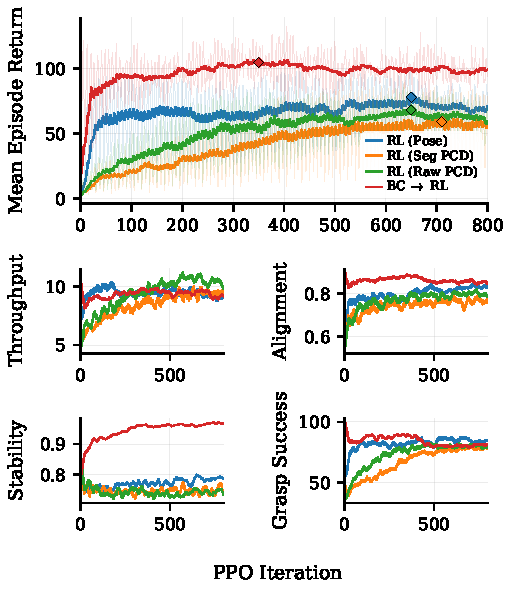
\includegraphics[width=\columnwidth]{reward_curves.pdf}
\caption{PPO training curves. Mean episode return (the cumulative per-grasp reward
$r = g \cdot \alpha \cdot \varsigma$ summed over one 200-log clearing episode, averaged across
$N_{\text{env}}=20$ parallel environments) vs.\ PPO iteration. Each iteration collects
$4 N_{\text{env}}$ grasp cycles and performs one PPO update; bold lines show a 20-iteration
rolling average with raw data in light shading. Diamond markers indicate the checkpoint
selected for evaluation (highest mean return before degradation). Flat segments occur when
no episode has terminated since the last update. All three from-scratch RL variants (Pose,
Seg.\ PCD, Raw PCD) improve per-grasp reward but fail to achieve full pile clearing
(Table~\ref{tab:rl_ablation}). BC$\to$RL initializes from the trained BC policy and reaches
the highest mean return while maintaining near-complete clearing; performance degrades after
$\sim$500 iterations, motivating early stopping. Bottom panels decompose the reward signal
into its per-grasp components.}
\label{fig:reward_curves}
\end{figure}

\subsection{BC-Initialized RL Fine-Tuning}
\label{sec:bcrl}
To combine BC's full-trajectory coverage with RL's ability to optimize per-grasp metrics, we initialize a PPO agent from the trained BC policy and fine-tune with on-policy experience~\cite{rajeswaran2018learning, nair2018overcoming}.

The BC actor weights (PointNet encoder and actor MLP) are loaded into the PPO actor; the critic is initialized randomly and the optimizer starts fresh.
We use an \emph{asymmetric actor-critic}~\cite{pinto2018asymmetric}: the actor observes the raw point cloud (same as BC), while the critic is a trainable MLP that receives the privileged 128D pose state vector (top-$K$ log poses).
This asymmetry allows the critic to learn a more accurate value function from compact state information, while the actor retains the vision-based input it will use at deployment.

We freeze the BC-trained PointNet encoder during RL fine-tuning.
The asymmetric critic cannot propagate gradients through the encoder, so an unfrozen encoder drifts without constraint; fine-tuning the full network causes training collapse (Fig.~\ref{fig:bcrl_ablation}).

All other PPO hyperparameters remain identical to the from-scratch RL configuration (Section~\ref{sec:rl}); the only changes are the frozen encoder and a reduced initial policy noise $\sigma_0 = 0.05$ (vs.\ $1.0$ for from-scratch RL), which limits exploration to small perturbations around the BC mean.

\TODO{Insert BC$\to$RL pipeline figure. Left: BC phase (expert demos $\to$ PointNet encoder + actor MLP, trained end-to-end with MSE loss). Center: RL phase (frozen PointNet encoder $\to$ trainable actor head + asymmetric state-based critic, trained with PPO). Right: Inference (frozen encoder + fine-tuned actor, no critic).}
Higher noise causes gradual degradation ($\sigma_0 = 0.1$) or rapid collapse ($\sigma_0 = 0.3$), as shown in Fig.~\ref{fig:bcrl_ablation}.

\begin{figure*}[t]
\centering
\TODO{Insert screenshot of multiple parallel environments, each showing a crane above a rack with 200 logs in different randomized pile configurations (varying spawn patterns, row jitter, layer offsets). Should convey the domain randomization and parallelized training setup.}
\caption{The grasp-and-remove crane environment. Each parallel environment contains a log loader crane positioned above a rack with 200 cylindrical logs spawned in randomized configurations. At each step, the policy selects a grasp target and a fixed FSM controller executes the pick sequence.}
\label{fig:environment}
\end{figure*}

\begin{figure*}[t]
\centering
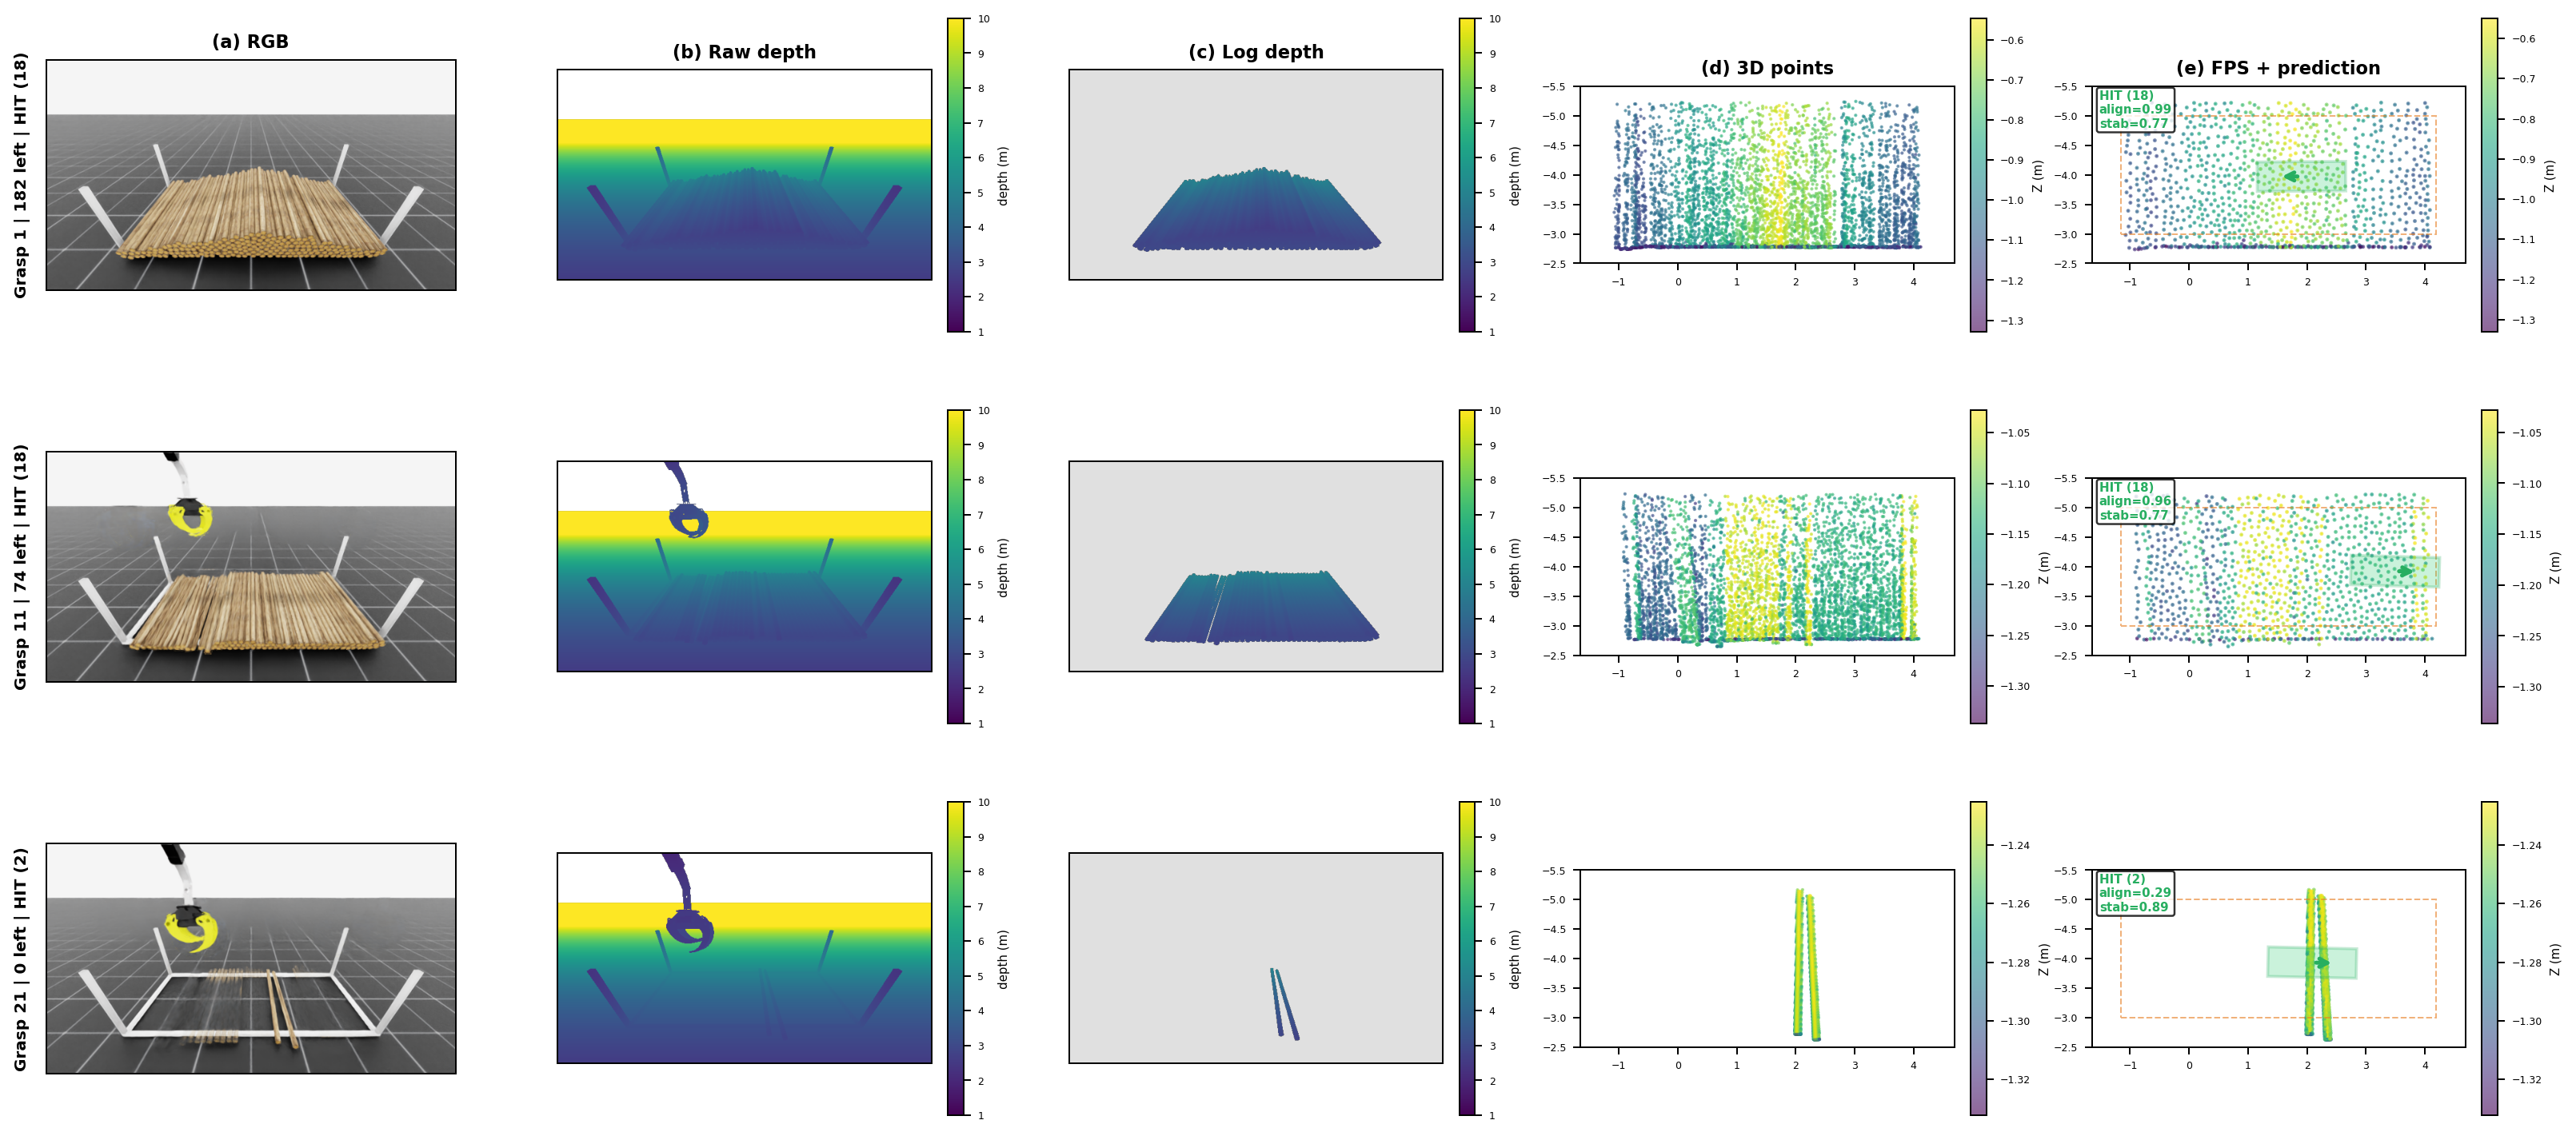
\includegraphics[width=\textwidth]{episode_001_pipeline.png}
\caption{Observation pipeline at three episode stages. Each row: (a)~RGB, (b)~depth, (c)~segmented depth, (d)~3D back-projection, (e)~FPS point cloud with predicted grasp target (green~=~hit, red~=~miss). Top: dense pile; middle: partially cleared; bottom: sparse endgame.}
\label{fig:pcd_pipeline}
\end{figure*}

\section{Experiments}
\subsection{Setup}
All experiments use the same crane model, rack geometry, and FSM controller, and run on a single NVIDIA RTX 4070 Laptop GPU (8\,GB VRAM).
Training uses 32 parallel environments for pose-based policies and 20 for point cloud policies (Fig.~\ref{fig:environment}).
Piles contain 200 cylindrical logs ($\sim$0.3\,m diameter, $\sim$3\,m length) spawned in layered grid patterns.
The log count is fixed across all experiments so that clearing metrics are directly comparable between methods; pile variation (Table~\ref{tab:robustness}) randomizes log count ($20$--$200$), grid dimensions, spacing ($\pm 5$--$15$\%), layer offsets, and per-log placement jitter to test generalization.

Each episode runs for a fixed budget of $H=30$ grasp attempts (see Section~\ref{sec:formulation} for the horizon rationale).
An episode terminates early if no logs remain on the rack (whether grasped or knocked out of bounds), though only intentionally grasped logs count toward the clearing rate.
For evaluation, we run 100 episodes (distributed across 20 parallel environments) on identical random seeds to ensure each method faces the same pile configurations.
All metrics are reported as per-episode mean $\pm$ standard deviation.
Training reward curves (Fig.~\ref{fig:reward_curves}) show single training runs; the reported variability comes from averaging over episodes within a run rather than across independent seeds.

\subsection{Metrics}
\label{sec:metrics}
We report per-grasp and per-episode metrics derived from the outcome evaluation tuple $(g, \alpha, \varsigma)$ defined in Section~\ref{sec:outcome}. All are reported as per-episode mean $\pm$ standard deviation unless noted:
\begin{itemize}
    \item Grasp success rate: fraction of grasps with $g>0$.
    \item Throughput: mean logs grasped per successful grasp.
    \item Alignment: grasp-count-weighted mean $\alpha \in [0,1]$ per episode (grasps capturing more logs contribute proportionally more).
    \item Stability: mean $\varsigma \in [0,1]$ over successful grasps per episode.
    \item Pile clearing rate: fraction of initial logs intentionally grasped and removed by episode end (knocked-off logs are excluded).
    \item Knocked-off percentage: fraction of initial logs knocked outside workspace bounds.
\end{itemize}
Our primary visualization is the clearing progression curve: for each method, we plot fraction of pile cleared (mean $\pm$ std across episodes) as a function of grasp attempt number (Fig.~\ref{fig:clearing_curves}).
This curve captures the full clearing dynamics, including where methods diverge and where RL plateaus.

\section{Results}
\label{sec:results}
\begin{table*}[t]
\centering
\caption{Evaluation results across 100 episodes with randomized 200-log pile configurations (mean $\pm$ std). All learned methods use raw point cloud observations processed by a PointNet encoder. RL uses a symmetric actor-critic (shared encoder); BC+RL uses an asymmetric actor-critic (frozen BC encoder for actor, state-based MLP critic).}
\label{tab:results}
\setlength{\tabcolsep}{5pt}
\begin{tabular}{@{}llcccccc@{}}
\toprule
Method & Obs. & Thru.\,$g$ & Align.\,$\alpha$ & Stab.\,$\varsigma$ & Grasp succ.\,(\%) & Clear rate\,(\%) & Knocked off\,(\%) \\
\midrule
Heuristic & Pose & $\mathbf{9.94 \pm 1.17}$ & $\mathbf{0.918 \pm 0.031}$ & $0.797 \pm 0.018$ & $\mathbf{88.7 \pm 7.8}$ & $99.0 \pm 1.2$ & $1.0 \pm 1.1$ \\
\addlinespace
RL        & Raw PCD & $6.78 \pm 1.01$ & $0.758 \pm 0.072$ & $0.815 \pm 0.039$ & $53.3 \pm 8.7$ & $53.0 \pm 3.9$ & $0.6 \pm 0.6$ \\
\addlinespace
BC        & Raw PCD & $9.32 \pm 1.12$ & $0.904 \pm 0.037$ & $0.824 \pm 0.025$ & $84.5 \pm 9.8$ & $\mathbf{98.5 \pm 5.1}$ & $\mathbf{0.7 \pm 0.7}$ \\
\addlinespace
BC$\to$RL & Raw PCD & $8.65 \pm 0.97$ & $0.906 \pm 0.027$ & $\mathbf{0.947 \pm 0.016}$ & $86.3 \pm 8.5$ & $98.2 \pm 1.5$ & $1.2 \pm 0.8$ \\
\bottomrule
\end{tabular}
\end{table*}

\begin{figure}[t]
\centering
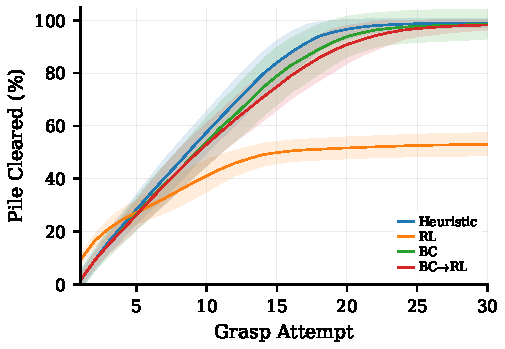
\includegraphics[width=\columnwidth]{clearing_curves.pdf}
\caption{Clearing progression: fraction of 200-log pile cleared vs.\ grasp attempt number (mean $\pm$ std over 100 episodes). RL plateaus at $\sim$53\% while BC, BC+RL, and the heuristic all approach full clearing.}
\label{fig:clearing_curves}
\end{figure}

Table~\ref{tab:results} summarizes the evaluation metrics.
All four methods share the same controller, pile configuration, and evaluation protocol; the only differences are the targeting policy and its observation.
From-scratch RL uses a symmetric actor-critic in which both actor and critic process observations through independent encoders (PointNet for PCD variants, MLPs for the pose ablation).
BC+RL uses an asymmetric actor-critic~\cite{pinto2018asymmetric} in which the actor retains the frozen BC-trained PointNet encoder while the critic is a trainable MLP that receives the privileged state vector (Section~\ref{sec:bcrl}).

\subsection{BC+RL Performance}
\label{sec:bcrl_perf}
BC+RL fine-tuning improves grasp stability by 15\% while preserving BC's full-trajectory clearing ability (Table~\ref{tab:results}).
BC+RL surpasses both BC and the privileged-state heuristic in stability by a wide margin, suggesting that RL optimizes the vertical component of grasp targets to produce more level lifts.
Alignment remains comparable to BC, so the quality improvement is driven entirely by more stable grasps.
Throughput is slightly lower, indicating that BC+RL favors more conservative, reliable grasps over maximum-throughput grasps.

Both the frozen encoder and conservative noise are critical.
Figure~\ref{fig:bcrl_ablation} compares four BC+RL training configurations: freezing the encoder with $\sigma_0 \in \{0.05, 0.1, 0.3\}$ and fine-tuning the full network with $\sigma_0 = 0.05$.
Only the frozen-encoder, $\sigma_0 = 0.05$ configuration sustains clearing performance through training; higher noise causes gradual ($\sigma_0 = 0.1$) or rapid ($\sigma_0 = 0.3$) collapse, and unfreezing the encoder causes immediate feature drift regardless of noise level.

\begin{figure}[t]
\centering
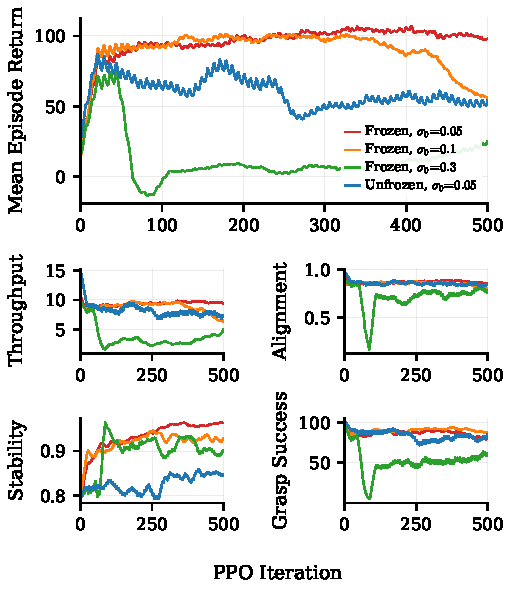
\includegraphics[width=\columnwidth]{bcrl_ablation.pdf}
\caption{BC+RL training sensitivity. Mean episode return vs.\ PPO iteration for four configurations varying encoder freezing and initial policy noise $\sigma_0$. Only the frozen-encoder, low-noise configuration ($\sigma_0 = 0.05$) sustains performance; all other variants collapse during training.}
\label{fig:bcrl_ablation}
\end{figure}

\subsection{BC Performance}
\label{sec:bc_perf}
BC achieves clearing comparable to the privileged-state heuristic using only raw point clouds (Table~\ref{tab:results}).
Conditional per-grasp metrics (throughput, alignment, stability) closely match the heuristic, indicating that the BC policy has captured the expert's targeting strategy: when a grasp succeeds, it is executed as effectively as one chosen with privileged state.
The main gap is in grasp success rate, concentrated in the endgame where sparse remaining logs are harder to localize from depth alone.
Despite more missed grasps, BC compensates by maintaining effective targeting throughout the clearing trajectory.

\subsection{RL Performance}
\label{sec:rl_perf}
From-scratch RL achieves competitive per-grasp reward during training (Fig.~\ref{fig:reward_curves}): RL~(Pose) converges to a mean episode reward of $\sim$95--97 within 80 iterations, while RL~(PCD) reaches $\sim$85--90 after 800+ iterations.
However, high training reward does not translate to pile-clearing performance.

To test whether observation type affects performance, we trained three RL variants with a symmetric actor-critic: privileged pose observations (128D), segmented PCD, and raw PCD.
All achieve roughly similar clearing (Table~\ref{tab:rl_ablation}), confirming that RL's failure is fundamental to the exploration landscape rather than a limitation of the observation representation.
In contrast, observation type does matter for BC: raw PCD outperforms segmented PCD in both clearing and success rate (Table~\ref{tab:rl_ablation}), showing that segmentation provides no benefit and slightly hurts performance.

\begin{table*}[t]
\centering
\caption{Observation type ablation for RL and BC. All RL variants use symmetric actor-critic. BC variants use PointNet with identical architecture. Metrics are mean $\pm$ std over 100 episodes. RL fails regardless of observation type; for BC, raw PCD outperforms segmented PCD across all metrics.}
\label{tab:rl_ablation}
\setlength{\tabcolsep}{5pt}
\begin{tabular}{@{}llcccccc@{}}
\toprule
Method & Obs. & Thru.\,$g$ & Align.\,$\alpha$ & Stab.\,$\varsigma$ & Grasp succ.\,(\%) & Clear rate\,(\%) & Knocked off\,(\%) \\
\midrule
RL & Pose (128D) & $8.84 \pm 1.68$ & $0.908 \pm 0.040$ & $0.970 \pm 0.021$ & $38.5 \pm 13.5$ & $49.4 \pm 14.8$ & $0.0 \pm 0.2$ \\
RL & Seg.\ PCD   & $7.04 \pm 1.06$ & $0.726 \pm 0.077$ & $0.776 \pm 0.042$ & $53.7 \pm 10.9$ & $55.2 \pm 5.4$ & $0.9 \pm 0.7$ \\
RL & Raw PCD     & $6.78 \pm 1.01$ & $0.758 \pm 0.072$ & $0.815 \pm 0.039$ & $53.3 \pm 8.7$ & $53.0 \pm 3.9$ & $0.6 \pm 0.6$ \\
\addlinespace
BC & Seg.\ PCD   & $9.64 \pm 1.05$ & $0.907 \pm 0.028$ & $0.816 \pm 0.020$ & $70.3 \pm 10.6$ & $96.5 \pm 4.7$ & $0.9 \pm 1.0$ \\
BC & Raw PCD     & $9.32 \pm 1.12$ & $0.904 \pm 0.037$ & $0.824 \pm 0.025$ & $84.5 \pm 9.8$ & $98.5 \pm 5.1$ & $0.7 \pm 0.7$ \\
\bottomrule
\end{tabular}
\end{table*}

The RL policies converge to narrow targeting patterns that yield adequate per-grasp reward in dense configurations but fail to adapt as the pile thins.
The best RL variant (Raw PCD) achieves only 53\% clearing with 53.3\% grasp success, compared to 98.5\% and 84.5\% for BC (Table~\ref{tab:rl_ablation}).

\begin{table*}[t]
\centering
\caption{Generalization under pile variation (mean $\pm$ std over 100 episodes). Each episode samples a random pile: log count uniform in $[20, 200]$, grid dimensions ($15$--$25$ columns, $10$--$20$ layers), lateral and vertical spacing ($\pm 5$--$15$\% of nominal), randomized layer offsets ($\pm 5$\,cm), and per-log placement jitter ($\pm 4$\,cm lateral, $\pm 2$\,cm vertical).}
\label{tab:robustness}
\setlength{\tabcolsep}{5pt}
\begin{tabular}{@{}llcccccc@{}}
\toprule
Method & Condition & Thru.\,$g$ & Align.\,$\alpha$ & Stab.\,$\varsigma$ & Grasp succ.\,(\%) & Clear rate\,(\%) & Knocked off\,(\%) \\
\midrule
Heuristic & Nominal        & $9.94 \pm 1.17$ & $0.918 \pm 0.031$ & $0.797 \pm 0.018$ & $88.7 \pm 7.8$  & $99.0 \pm 1.2$ & $1.0 \pm 1.1$ \\
Heuristic & Pile variation & $8.28 \pm 1.96$ & $0.889 \pm 0.074$ & $0.789 \pm 0.024$ & $86.3 \pm 11.6$ & $98.2 \pm 4.9$ & $1.3 \pm 1.6$ \\
\addlinespace
BC        & Nominal        & $9.32 \pm 1.12$ & $0.904 \pm 0.037$ & $0.824 \pm 0.025$ & $84.5 \pm 9.8$  & $98.5 \pm 5.1$ & $0.7 \pm 0.7$ \\
BC        & Pile variation & $7.55 \pm 2.02$ & $0.860 \pm 0.093$ & $0.820 \pm 0.029$ & $72.8 \pm 17.7$ & $98.4 \pm 2.5$ & $1.2 \pm 1.5$ \\
\addlinespace
BC$\to$RL & Nominal        & $8.65 \pm 0.97$ & $0.906 \pm 0.027$ & $0.947 \pm 0.016$ & $86.3 \pm 8.5$  & $98.2 \pm 1.5$ & $1.2 \pm 0.8$ \\
BC$\to$RL & Pile variation & $6.97 \pm 1.63$ & $0.861 \pm 0.081$ & $0.922 \pm 0.037$ & $76.0 \pm 14.9$ & $98.5 \pm 1.5$ & $1.3 \pm 1.4$ \\
\bottomrule
\end{tabular}
\end{table*}

\begin{figure*}[t]
\centering
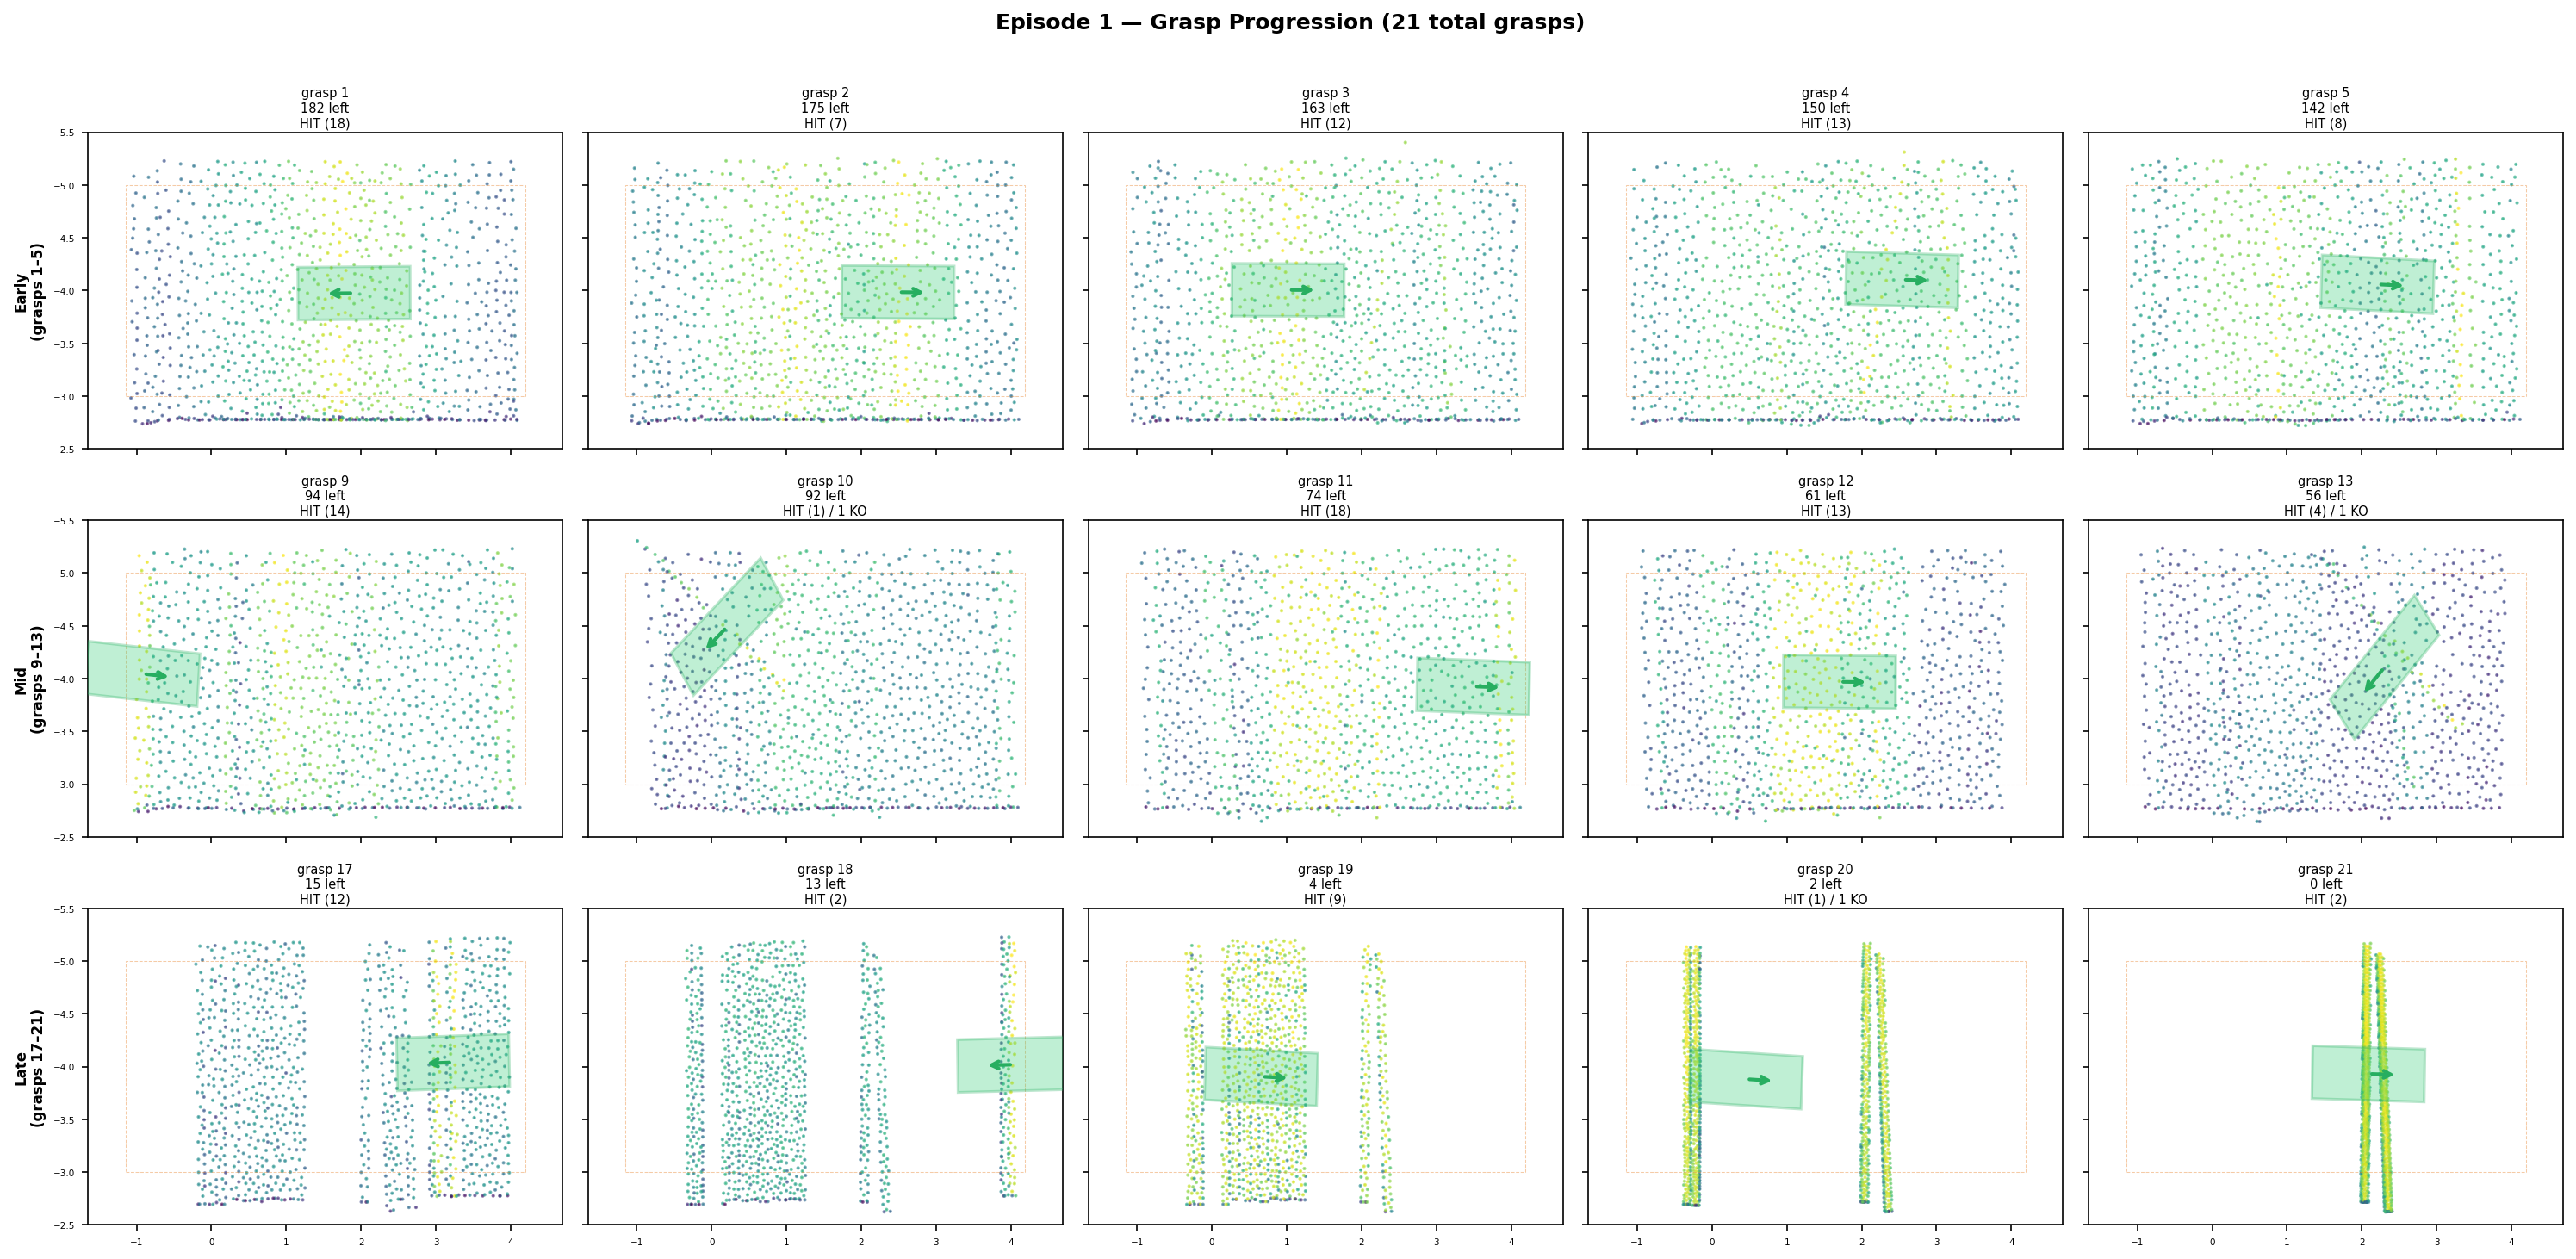
\includegraphics[width=\textwidth]{episode_001_progression.png}
\caption{Grasp progression for a single BC (PCD) episode clearing 200 logs in 21 grasps. Each panel shows the FPS-downsampled point cloud with the predicted grasp target (green rectangle). Top row: early grasps into the dense pile; middle row: mid-episode with thinning pile; bottom row: endgame grasps targeting sparse remaining logs. The pile transitions from a dense ordered stack to a thin irregular layer.}
\label{fig:progression}
\end{figure*}

\section{Discussion and Limitations}

The clearing progression (Fig.~\ref{fig:clearing_curves}) reveals a clear divergence around grasp 5--10: from-scratch RL throughput drops steadily and plateaus near 53\%, while the heuristic, BC, and BC+RL maintain similar clearing rates through the full episode. The near-identical clearing curves of BC and BC+RL confirm that RL fine-tuning preserves the expert's clearing ability while improving grasp stability (Table~\ref{tab:results}).

From-scratch RL achieves competitive per-grasp reward but stalls at roughly 53\% clearing regardless of observation type (Table~\ref{tab:rl_ablation}).
Because the per-grasp reward provides no direct incentive for global clearing, the policy converges to a narrow targeting pattern that yields adequate reward in dense configurations but does not adapt as the pile geometry changes through clearing.
Once the easily accessible logs are exhausted, the fixed strategy produces missed grasps that consume the episode budget.
This failure is not a perception limitation. RL with privileged pose observations fares no better. Rather, it is a consequence of the exploration landscape: the policy never discovers the full diversity of pile states encountered during a complete clearing trajectory.
We also evaluated three reward shaping strategies (Table~\ref{tab:reward_ablation}): removing quality terms to simplify the reward landscape, normalizing throughput by available logs, and combining tiered clearing bonuses (at 60/75/90\%) with pile-size curriculum. All variants achieved comparable or higher per-grasp reward but none resolved the clearing plateau, suggesting that the bottleneck is exploration rather than reward design.

\begin{table}[t]
\centering
\caption{Reward shaping ablation. All variants use raw PCD observations
with from-scratch RL (500 iterations, 20 parallel environments).
None resolves the clearing plateau exhibited by the baseline.}
\label{tab:reward_ablation}
\setlength{\tabcolsep}{3pt}
\begin{tabular}{lc}
\toprule
Variant & Clear.\,\% \\
\midrule
Baseline ($g \cdot \alpha \cdot \varsigma$) & 53.0 \\
Throughput only ($g$) & TBD \\
Normalized ($\frac{g}{\text{avail}} \cdot \alpha \cdot \varsigma$) & TBD \\
Curriculum + bonus@60/75/90\% & TBD \\
\bottomrule
\end{tabular}
\end{table}

BC initialization provides exactly the coverage that from-scratch RL lacks: the demonstration data spans the full clearing trajectory from dense stacks to sparse endgames~\cite{rajeswaran2018learning}.
RL fine-tuning then optimizes per-grasp execution quality without needing to rediscover the global targeting strategy.
The stability improvement suggests that RL learns to refine the vertical positioning of grasps, producing more level lifts.
Freezing the BC-trained encoder is critical to prevent feature drift, since the state-based critic provides no gradient signal to the visual pathway (Section~\ref{sec:bcrl}).
The low initial noise ($\sigma_0 = 0.05$) further prevents the RL updates from overwriting the BC-learned policy.

Raw point clouds achieve comparable clearing via both BC and BC+RL, matching or exceeding the segmented-PCD baseline (Table~\ref{tab:rl_ablation}).
This has practical implications for sim-to-real transfer: removing the dependency on a trained segmentation model simplifies the perception pipeline and eliminates a potential failure mode.
The PointNet encoder learns to extract task-relevant geometry directly from the raw depth signal.

BC+RL grasps slightly fewer logs per attempt than BC but compensates with a higher success rate, maintaining the same clearing performance.
The stability improvement is a pure gain: BC+RL produces substantially more level lifts without sacrificing clearing ability.

All three methods maintain near-complete clearing under pile variation (Table~\ref{tab:robustness}), with randomized log counts, spawn patterns, and stacking offsets.
Throughput and grasp success decrease for all methods on varied piles, as smaller or irregularly shaped piles present fewer easy multi-log grasps.
The learned policies show a larger success rate drop than the heuristic, likely because the BC demonstrations were collected on fixed 200-log piles, so the policy has less coverage of smaller pile configurations.

Our grasp-and-remove design isolates targeting and enables fast experimentation, but has limitations.
First, grasp success is approximated by proximity after lift, rather than explicit contact constraints.
Second, removed logs are teleported rather than placed, so the task omits deposition planning and re-contact dynamics.
Third, the PointNet encoder operates on unordered point sets without explicit spatial structure; architectures that exploit local geometry (e.g., PointNet++~\cite{qi2017pointnetplusplus}, point transformers) may improve endgame targeting.
Fourth, all experiments are in simulation; sim-to-real transfer is a natural next step.
Despite these simplifications, the environment captures the essential challenges of sequential multi-log grasping from dense piles.

\section{Conclusion}
We presented a grasp-and-remove crane environment for studying grasp target selection in dense log-pile clearing at scale, and compared four methods (heuristic, from-scratch RL, BC, and BC+RL) on a shared controller and evaluation protocol.
Our results show that from-scratch RL fails to clear dense piles regardless of observation type, stalling at roughly 53\%.
BC trained on raw point clouds achieves clearing comparable to the privileged-state heuristic.
BC+RL fine-tuning improves grasp stability by 15\% over BC while maintaining near-complete clearing, demonstrating that demonstration data provides the exploration curriculum that RL cannot discover on its own.
The success of raw point clouds simplifies the perception pipeline for future sim-to-real transfer.
Future work will explore sim-to-real deployment with physics domain randomization, and richer point cloud architectures (e.g., PointNet++, point transformers).

\section*{ACKNOWLEDGMENT}
[Redacted for anonymity]

\bibliographystyle{IEEEtran}
\bibliography{references}

\end{document}
